%\documentclass[10pt,handout]{beamer}
\documentclass[10pt]{beamer}\usepackage[]{graphicx}\usepackage[]{color}
%% maxwidth is the original width if it is less than linewidth
%% otherwise use linewidth (to make sure the graphics do not exceed the margin)
\makeatletter
\def\maxwidth{ %
  \ifdim\Gin@nat@width>\linewidth
    \linewidth
  \else
    \Gin@nat@width
  \fi
}
\makeatother

\definecolor{fgcolor}{rgb}{0.345, 0.345, 0.345}
\newcommand{\hlnum}[1]{\textcolor[rgb]{0.686,0.059,0.569}{#1}}%
\newcommand{\hlstr}[1]{\textcolor[rgb]{0.192,0.494,0.8}{#1}}%
\newcommand{\hlcom}[1]{\textcolor[rgb]{0.678,0.584,0.686}{\textit{#1}}}%
\newcommand{\hlopt}[1]{\textcolor[rgb]{0,0,0}{#1}}%
\newcommand{\hlstd}[1]{\textcolor[rgb]{0.345,0.345,0.345}{#1}}%
\newcommand{\hlkwa}[1]{\textcolor[rgb]{0.161,0.373,0.58}{\textbf{#1}}}%
\newcommand{\hlkwb}[1]{\textcolor[rgb]{0.69,0.353,0.396}{#1}}%
\newcommand{\hlkwc}[1]{\textcolor[rgb]{0.333,0.667,0.333}{#1}}%
\newcommand{\hlkwd}[1]{\textcolor[rgb]{0.737,0.353,0.396}{\textbf{#1}}}%
\let\hlipl\hlkwb

\usepackage{framed}
\makeatletter
\newenvironment{kframe}{%
 \def\at@end@of@kframe{}%
 \ifinner\ifhmode%
  \def\at@end@of@kframe{\end{minipage}}%
  \begin{minipage}{\columnwidth}%
 \fi\fi%
 \def\FrameCommand##1{\hskip\@totalleftmargin \hskip-\fboxsep
 \colorbox{shadecolor}{##1}\hskip-\fboxsep
     % There is no \\@totalrightmargin, so:
     \hskip-\linewidth \hskip-\@totalleftmargin \hskip\columnwidth}%
 \MakeFramed {\advance\hsize-\width
   \@totalleftmargin\z@ \linewidth\hsize
   \@setminipage}}%
 {\par\unskip\endMakeFramed%
 \at@end@of@kframe}
\makeatother

\definecolor{shadecolor}{rgb}{.97, .97, .97}
\definecolor{messagecolor}{rgb}{0, 0, 0}
\definecolor{warningcolor}{rgb}{1, 0, 1}
\definecolor{errorcolor}{rgb}{1, 0, 0}
\newenvironment{knitrout}{}{} % an empty environment to be redefined in TeX

\usepackage{alltt}
\usepackage{etex} % helps fix \newdimen error which is cause when ctable is loaded with other packages
\usepackage{comment}
\usepackage{amsmath,amsthm,amssymb}
\usepackage{url}
\usepackage{color, colortbl}
\usepackage{tikz}
\usepackage{ctable}

\usetikzlibrary{shapes.geometric, arrows,shapes.symbols,decorations.pathreplacing}
\tikzstyle{startstop} = [rectangle, rounded corners, minimum width=3cm, minimum height=1cm, draw=black, fill=pinkish,text width=3.5cm]
\tikzstyle{startstop2} = [rectangle, rounded corners, minimum width=3cm, minimum height=1cm, draw=black, fill=background,text width=4.5cm]
\tikzstyle{startstop3} = [rectangle, rounded corners, minimum width=3cm, minimum height=1cm, draw=black, fill=beige,text width=3.0cm]
\tikzstyle{startstop4} = [rectangle, rounded corners, minimum width=3cm, minimum height=1cm, draw=black, fill=pinkish,text width=4.5cm]
\tikzstyle{io} = [trapezium, trapezium left angle=70, trapezium right angle=110, minimum width=2cm, minimum height=1cm, text centered, draw=black, fill=blue!30,text width=1.5cm]
\tikzstyle{process} = [rectangle, minimum width=1cm, minimum height=1cm, text centered, draw=black, fill=orange!30,text width=2cm]
\tikzstyle{decision} = [diamond, minimum width=2cm, minimum height=1cm, text centered, draw=black, fill=green!30]
\tikzstyle{arrow} = [thick,->,>=stealth]
\tikzstyle{both} = [thick,<->,>=stealth, red]
% define a bunch of colors
\definecolor{gray}{RGB}{110,110,110}
\definecolor{darkgray}{RGB}{100,100,100}
\definecolor{lightgray}{RGB}{200,200,200}
\definecolor{turquoise}{RGB}{81,193,188}
\definecolor{tomato}{RGB}{255,136,136}
\definecolor{mandarina}{RGB}{229,169,25}
\definecolor{foreground}{RGB}{81,141,193}
\definecolor{background}{RGB}{246,244,240}
\definecolor{highlight}{RGB}{229,169,25}
\definecolor{lowlight}{RGB}{200,200,200}
\definecolor{beige}{RGB}{255,255,240}
\definecolor{pinkish}{RGB}{255,223,247}

\tikzset{myshade/.style={minimum size=.4cm,shading=radial,inner color=white,outer color={#1!90!gray}}}
\newcommand\mycirc[1][]{\tikz\node[circle,myshade=#1]{};}
\newcommand\myrect[1][]{\tikz\node[rectangle,myshade=#1]{};}
\newcommand\mystar[1][]{\tikz\node[star,star points=15,star point height=2pt,myshade=#1]{};}
\newcommand\mydiamond[1][]{\tikz\node[diamond,myshade=#1]{};}
\newcommand\myellipse[1][]{\tikz\node[ellipse,myshade=#1]{};}
\newcommand\mykite[1][]{\tikz\node[kite,myshade=#1]{};}
\newcommand\mydart[1][]{\tikz\node[dart,myshade=#1]{};}
\newcommand\mycloud[1][]{\tikz\node[cloud,myshade=#1]{};}

%\usepackage{subcaption}
\usepackage{subfig}
%\usepackage{caption}

\mode<presentation>
\usetheme{Hannover}
\usecolortheme{rose}
\setbeamertemplate{navigation symbols}{}
\setbeamertemplate{footline}[frame number]
\setbeamertemplate{caption}[numbered]
\setbeamertemplate{frametitle}[default][left]

\usepackage{fontspec}
%\setsansfont{Fira Sans}
%\setmonofont{Fira Mono}
\setsansfont[ItalicFont={Fira Sans Light Italic},BoldFont={Fira Sans},BoldItalicFont={Fira Sans Italic}]{Fira Sans Light}
\setmonofont[BoldFont={Fira Mono Medium}]{Fira Mono}

\usepackage[]{hyperref}
\hypersetup{
    unicode=false,          
    pdftoolbar=true,        
    pdfmenubar=true,        
    pdffitwindow=false,     % window fit to page when opened
    pdfstartview={FitH},    % fits the width of the page to the window
    pdftitle={Reproducible Research},    % title
    pdfauthor={Sahir Rai Bhatnagar},     % author
    pdfsubject={Subject},   % subject of the document
    pdfcreator={Sahir Rai Bhatnagar},   % creator of the document
    pdfproducer={Sahir Rai Bhatnagar}, % producer of the document
    pdfkeywords={}, % list of keywords
    pdfnewwindow=true,      % links in new window
    colorlinks=true,       % false: boxed links; true: colored links
    linkcolor=red,          % color of internal links (change box color with linkbordercolor)
    citecolor=blue,        % color of links to bibliography
    filecolor=black,      % color of file links
    urlcolor=cyan           % color of external links
}


\newcommand{\code}[1]{\texttt{#1}}


\AtBeginSection[]{
	\begin{frame}
	\vfill
	\centering
	\begin{beamercolorbox}[sep=8pt,center,shadow=true,rounded=true]{title}
		\usebeamerfont{title}\insertsectionhead\par%
	\end{beamercolorbox}
	\vfill
\end{frame}
}
\IfFileExists{upquote.sty}{\usepackage{upquote}}{}
\begin{document}






\title[Outils pour la diffusion rapide et reproductible de la recherche]{Avoir une présence en ligne}
\subtitle{Outils pour la diffusion rapide et reproductible de la recherche}

\author[]{Sahir Rai Bhatnagar%
\thanks{\href{https://github.com/sahirbhatnagar/raqc}{https://github.com/sahirbhatnagar/raqc}%
}}

\date{May 14, 2019}

%\makebeamertitle

\maketitle

\begin{frame}{Remerciements}
% \hspace*{-1.9cm}\parbox[t]{\textwidth}
%\frametitle{Acknowledgements}
\begin{columns}[c] % The "c" option specifies centered vertical alignment while the "t" option is used for top vertical alignment

\column{.45\textwidth} % Left column and width

\begin{itemize}
%\scriptsize
\item La comité organisateur
\item Pierre Racine et Sophie Baillargeon
\item Don Knuth (\TeX)
\item Friedrich Leisch (Sweave)
\item Yihui Xie (knitr)
\item Vous
\end{itemize}

\column{.45\textwidth} % Right column and width
\begin{figure}

\includegraphics[width=1.0\columnwidth]{logo_r_a_quebec_2019_presente_par_ia_blanc.png}\\[5mm]

\includegraphics[width=1.0\columnwidth]{ulaval-logo.jpg}
%\includegraphics[width=0.7\columnwidth]{Logo-LUDMER.jpg}
\end{figure}

\end{columns}
\end{frame}


\begin{frame}{Avis \#1}
\begin{itemize}
	\item Ceci est une \textbf{introduction} au outils pour la recherche reproductible
	\pause \item Le niveau de cet atelier est "intermédiaire" et suppose des connaissances de base en R ainsi que de l'environnement RStudio
	%\pause \item On va faire beaucoup d'exercices
	\pause \item N'h\'{e}sitez pas \`{a} posez des questions
\end{itemize}
\end{frame}


\begin{frame}{Avis \#2}
\begin{figure}

\includegraphics[width=1.0\columnwidth]{rstudio.png}\\[5mm]

\includegraphics[width=0.2\columnwidth]{rlogo.png}\\[5mm]

\includegraphics[width=0.2\columnwidth]{LaTeX_logo.png}
\end{figure}

\textit{Je n'ai aucune relation commerciale avec ces logiciels.}

\end{frame}

\begin{frame}{Avis \#3}

\begin{itemize}
\item Le mat\'{e}riel pour cet atelier est bas\'{e} sur plusieurs ressources 
\item Voir ce lien pour une liste compl\`{e}te de r\'{e}f\'{e}rences: \href{https://github.com/sahirbhatnagar/raqc}{https://github.com/sahirbhatnagar/raqc}
\item Une grande partie du contenu de ces diapositives est basée sur ces deux livres:
\end{itemize}

\begin{columns}[c] % The "c" option specifies centered vertical alignment while the "t" option is used for top vertical alignment
\column{.45\textwidth} % Left column and width
\begin{figure}
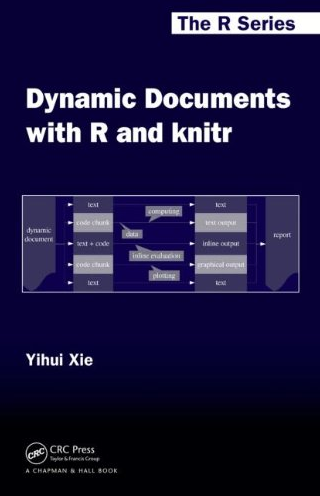
\includegraphics[width=0.6\columnwidth]{yihui.png}
\end{figure}

\column{.45\textwidth} % Right column and width
\begin{figure}

\includegraphics[width=0.6\columnwidth]{blogdown.png}
\end{figure}
\end{columns}

\end{frame}


\begin{frame}{Eat Your Own Dog Food}

\begin{itemize}
\item Ces diapositives sont reproductibles
\item Voir \texttt{raqc-slides.Rnw}: \href{https://github.com/sahirbhatnagar/raqc/tree/master/slides}{https://github.com/sahirbhatnagar/raqc/tree/master/slides}
\end{itemize}

\end{frame}



\begin{frame}{Le programme de l'atelier}
\begin{itemize}
\item \textbf{8h30 à 10h00}: Introduction aux raports reproductibles avec knitr et RMarkdown
\item \textbf{10h00 à 10h30}: Pause
\item \textbf{10h30 à 12h00}: 
\item \textbf{13h30 à 15h00}: Créer un siteweb avec blogdown
\item \textbf{15h00 à 15h30}: Pause
\item \textbf{15h30 à 17h}: 
\item \textbf{17h}: Fin de l'atelier
\end{itemize}
\end{frame}



\section{Recherche Reproductible (RR)}

\subsection{Quoi?}

\begin{frame}

\frametitle{C'est quoi la science?}

\pause
\begin{block}{Selon l'American Physical Society:}
La science est l'entreprise systématique consistant à rassembler des connaissances sur l'univers et à les organiser et les condenser en lois et \textbf{théories vérifiables}... \\ \pause
\vspace*{0.2in}	
Le \textbf{succès et la crédibilité de la science} sont fondés sur la volonté des scientifiques \textbf{d'exposer leurs idées} et \textbf{leurs résultats} à des \textbf{tests indépendants} et à leur \textbf{reproduction} par d'autres scientifiques.

\end{block}

\end{frame}

%%%%%%%%%%%%%%%%%%%%%%%%%%%%%%%%%%%%%%%%%%%%%%%%%%%%%%%%%%%%%%%%%%%%%%%%%%%%%%%%%%%%%%%%%%%%%
\begin{frame}

\frametitle{RR: Une norme minimale pour vérifier les résultats scientifiques}

\pause
\begin{block}{Recherche reproductible (RR) dans la science des données}
Les données et le code utilisés pour effectuer une constatation sont disponibles et suffisent à un chercheur indépendant pour recréer la constatation.
\end{block}

\end{frame}

%%%%%%%%%%%%%%%%%%%%%%%%%%%%%%%%%%%%%%%%%%%%%%%%%%%%%%%%%%%%%%%%%%%%%%%%%%%%%%%%%%%%%%%%%%%%%
%%%%%%%%%%%%%%%%%%%%%%%%%%%%%%%%%%%%%%%%%%%%%%%%%%%%%%%%%%%%%%%%%%%%%%%%%%%%%%%%%%%%%%%%%%%%%

\subsection{Pourquoi?}

\begin{frame}
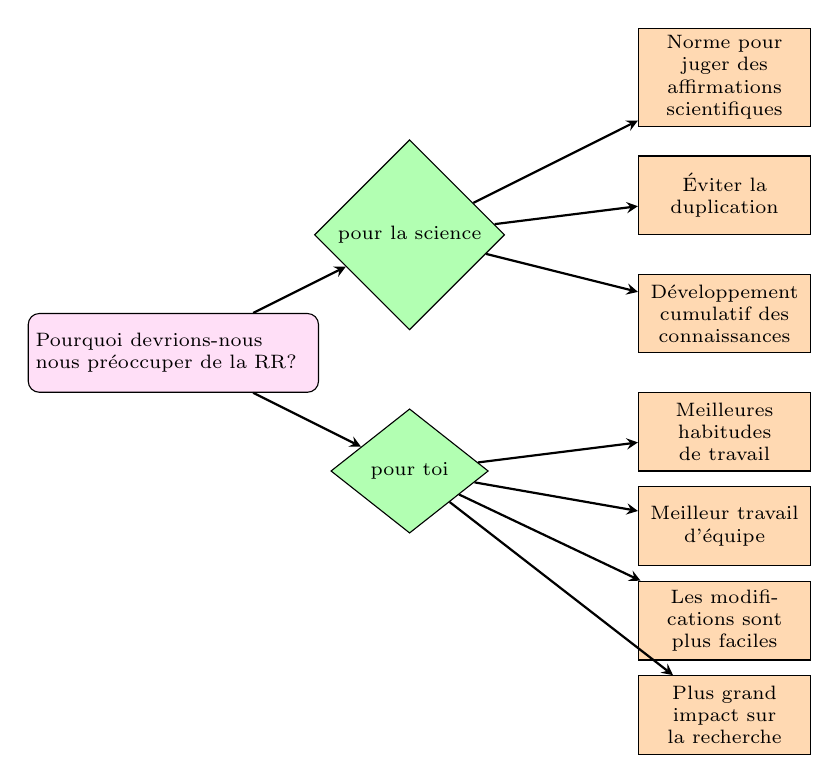
\begin{tikzpicture}
\scriptsize
\node (expr) [startstop] {Pourquoi devrions-nous nous préoccuper de la RR?};
\node (science) [decision, right of=expr, xshift=2cm, yshift=1.5cm] {pour la science};
\draw [arrow] (expr) -- (science);
\node (stan) [process, right of=science, xshift=3cm, yshift=2cm] {Norme pour juger des affirmations scientifiques};
\node (dupli) [process, right of=science, xshift=3cm, yshift=0.5cm] {Éviter la duplication};
\node (know) [process, right of=science, xshift=3cm, yshift=-1cm] {Développement cumulatif des connaissances};
\draw [arrow] (science) -- (stan);
\draw [arrow] (science) -- (dupli);
\draw [arrow] (science) -- (know);
\pause \node (you) [decision, right of=expr, xshift=2cm, yshift=-1.5cm] {pour toi};
\draw [arrow] (expr) -- (you);
\node (work) [process, right of=you, xshift=3cm, yshift=0.5cm] {Meilleures habitudes de travail};
\node (team) [process, right of=you, xshift=3cm, yshift=-0.7cm] {Meilleur travail d'équipe};
\node (change) [process, right of=you, xshift=3cm, yshift=-1.9cm] {Les modifications sont plus faciles};
\node (soft) [process, right of=you, xshift=3cm, yshift=-3.1cm] {Plus grand impact sur la recherche};
\draw [arrow] (you) -- (work);
\draw [arrow] (you) -- (team);
\draw [arrow] (you) -- (change);
\draw [arrow] (you) -- (soft);
\end{tikzpicture}
\end{frame}


\subsection{001-exemple-justificatif}

\begin{frame}{Un exemple justificatif}
\textit{Démo:} \href{https://github.com/sahirbhatnagar/raqc/tree/master/001-motivating-example}{001-motivating-example}\\

%\textit{Survey:}
%\href{https://www.surveymonkey.com/s/CDVXW3C}{https://www.surveymonkey.com/s/CDVXW3C}
\end{frame}



\section{Commencer}

\begin{frame}{Outils pour la recherche reproductible\footnote{\href{http://onepager.togaware.com/}{http://onepager.togaware.com/}}}


\begin{block}{Logiciel gratuit et << open source >>}
\begin{itemize}
\item \texttt{RStudio}: Créer, gérer, compiler des documents
\item \LaTeX: langage de balisage pour la composition d'un document
\item \texttt{R}: Langage d'analyse statistique
\item \texttt{knitr}: Intègre le code \LaTeX et le code \texttt{R}. La version moderne de \href{https://www.statistik.lmu.de/~leisch/Sweave/}{\texttt {Sweave}} du professeur Friedrich Leisch
\item \texttt{RMarkdown}: Intègre le code Markdown et le code \texttt{R}
\end{itemize}
\end{block}
\end{frame}


\subsection{\LaTeX}

\begin{frame}\frametitle{Comparaison}
\begin{columns}[c] % The "c" option specifies centered vertical alignment while the "t" option is used for top vertical alignment

\column{.45\textwidth} % Left column and width
\begin{figure}[h!]
\centering
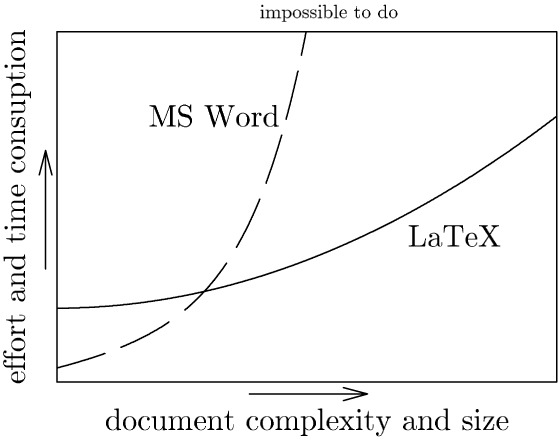
\includegraphics[scale=1, keepaspectratio]{./miktex}
\caption{Comparison}
\label{fig:word}
\end{figure}

\column{.5\textwidth} % Right column and width
\begin{itemize}
\item \LaTeX \, a une plus grande courbe d'apprentissage
\item De nombreuses tâches sont très difficiles ou impossibles (la plupart des cas) à effectuer dans MS Word ou Libre Office
\end{itemize}
\end{columns}

\end{frame}

%%%%%%%%%%%%%%%%%%%%%%%%%%%%%%%%%%%%%%%%%%%%%%%%%%%%%%%%%%%%%%%%%%%%%%%%%%%%%%%%%%%%%%%%%%%%%

\begin{frame}\frametitle{La philosophie derrière \LaTeX}
\begin{columns}[c] % The "c" option specifies centered vertical alignment while the "t" option is used for top vertical alignment

\column{.45\textwidth} % Left column and width
\begin{figure}[h!]
\centering
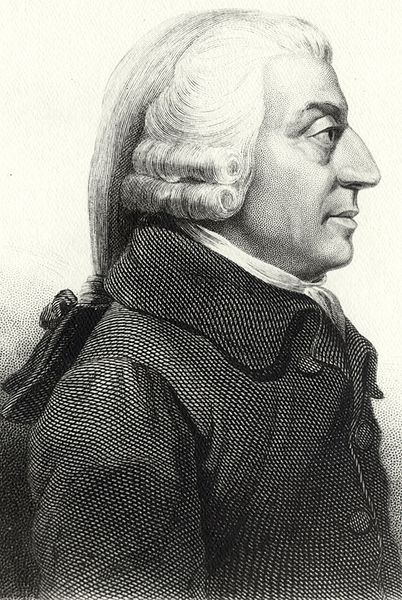
\includegraphics[scale=0.6, keepaspectratio]{./smith}
\small
\caption{Adam Smith, l'auteur de \textit{The Wealth of Nations} (1776), dans lequel il conceptualise la notion de division du travail}
\label{fig:smith}
\end{figure}

\column{.5\textwidth} % Right column and width
\small
\begin{block}{Division du travail}
La \textbf{composition} et la structuration logique du texte constituent la contribution spécifique de \textbf{l'auteur} à la production d'un texte imprimé. \\
\vspace*{0.25in}
\pause
Des questions telles que le choix de la famille de polices, les \textbf{en-têtes de section doivent-ils être en caractères gras ou en petites capitales}? Doivent-ils être alignés à gauche ou centrés? Le texte doit-il être justifié ou non? Les notes doivent-elles apparaître au bas de la page ou à la fin? Le texte doit-il être placé dans une colonne ou deux? et ainsi de suite, est l'affaire de la \textbf{typographe}
\end{block}
\end{columns}

\end{frame}

%%%%%%%%%%%%%%%%%%%%%%%%%%%%%%%%%%%%%%%%%%%%%%%%%%%%%%%%%%%%%%%%%%%%%%%%%%%%%%%%%%%%%%%%%%%%%

\begin{frame}\frametitle{Le génie derrière \LaTeX}

\begin{figure}[h!]
\centering
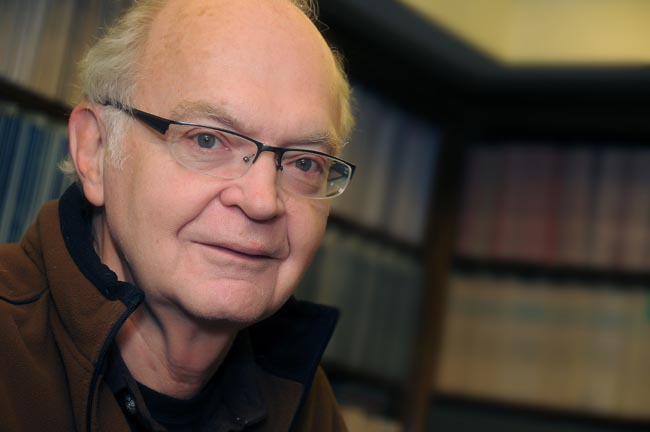
\includegraphics[scale=0.4, keepaspectratio]{./don}
\small
\caption{The \TeX~project was started in 1978 by Donald Knuth (Stanford). He planned for 6 months, but it took him nearly 10 years to complete. Coined the term ``Literate programming'': mixture of code and text segments that are ``human'' readable. Recipient of the Turing Award (1974) and the Kyoto Prize (1996).}
\label{fig:don}
\end{figure}

\end{frame}



\subsection{RStudio}

\begin{frame}\frametitle{Integrated Development Environment (IDE)}
\pause
\begin{figure}[h!]
\centering
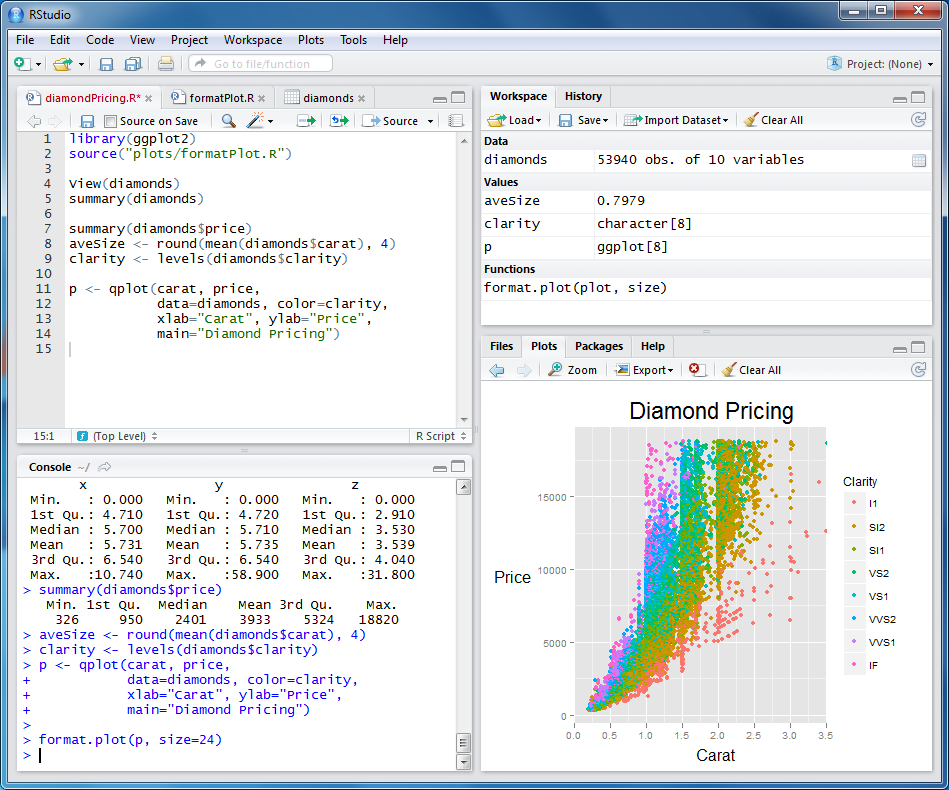
\includegraphics[scale=0.25, keepaspectratio]{./RStudio-Screenshot}
\end{figure}
\textit{Demonstrate:} Explore \texttt{RStudio} 
\end{frame}


\subsection{\texttt{knitr}}

\begin{frame}{Que fait \texttt{knitr}}
Exemple \textbf{\LaTeX}:

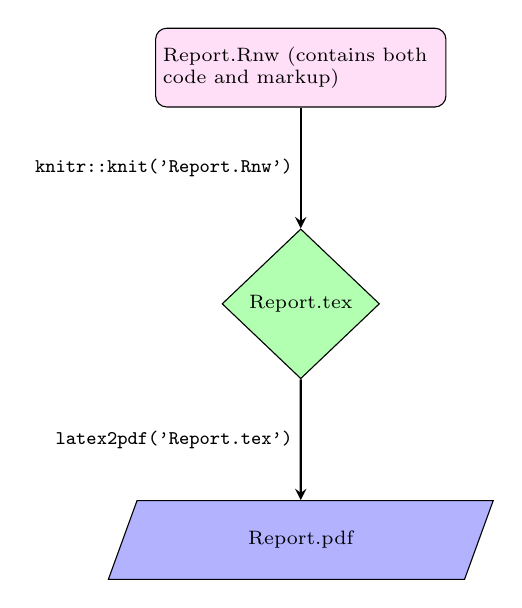
\begin{tikzpicture}
\scriptsize
\node (expr) [startstop] {Report.Rnw (contains both code and markup)};
\node (science) [decision, below of=expr, xshift=0cm, yshift=-2cm] {Report.tex};
\draw [arrow] (expr) -- node[anchor=east]{\texttt{knitr::knit('Report.Rnw')}} (science);
\pause \node (pdf) [io, below of=science, xshift=0cm, yshift=-2cm] {Report.pdf};
\draw [arrow] (science) -- node[anchor=east]{\texttt{latex2pdf('Report.tex')}} (pdf);
\end{tikzpicture}
\end{frame}


\begin{frame}\frametitle{Compiler un document \texttt{.Rnw}}

\begin{block}{Les deux étapes de la diapositive précédente peuvent être exécutées en une seule commande:}
\[ \textrm{\texttt{knitr::knit2pdf()}} \]
\end{block}

ou dans \texttt{RStudio}:
\begin{figure}[h!]
\centering
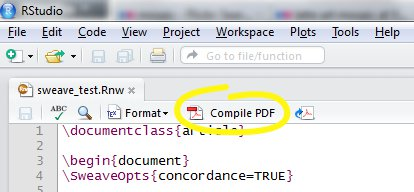
\includegraphics[scale=0.5, keepaspectratio]{./Compile-pdf.jpg}
\end{figure}
%\textit{Demonstrate:} Explore \texttt{RStudio}, projects and \texttt{.Rprofile}
\end{frame}

\begin{frame}\frametitle{Incorporer le code \texttt{R}}

\begin{itemize}
\item Insérer le code \texttt{R} dans un \textbf{morceau de code} commençant par $$ << \quad >>= $$
et se terminant par
\begin{center}
{@}
\end{center}
\end{itemize}

Dans \texttt{RStudio}:
\begin{figure}[h!]
\centering
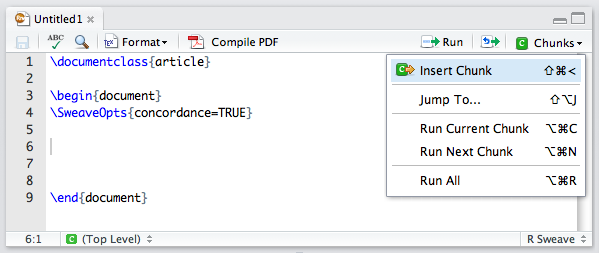
\includegraphics[scale=0.35, keepaspectratio]{./sweave_chunk}
\end{figure}
%\textit{Demonstrate:} Explore \texttt{RStudio}, projects and \texttt{.Rprofile}
\end{frame}

\begin{frame}[fragile]{Exemple 1}
\begin{knitrout}\footnotesize
\definecolor{shadecolor}{rgb}{0.969, 0.969, 0.969}\color{fgcolor}\begin{kframe}
\begin{verbatim}
<<example-code-chunk-name, echo=TRUE>>=
library(magrittr)
rnorm(50) %>% mean
@
\end{verbatim}
\end{kframe}
\end{knitrout}
produces
\begin{knitrout}\footnotesize
\definecolor{shadecolor}{rgb}{0.969, 0.969, 0.969}\color{fgcolor}\begin{kframe}
\begin{alltt}
\hlkwd{library}\hlstd{(magrittr)}
\hlkwd{rnorm}\hlstd{(}\hlnum{50}\hlstd{)} \hlopt \hlstd{mean}
\end{alltt}
\begin{verbatim}
## [1] 0.12
\end{verbatim}
\end{kframe}
\end{knitrout}
\end{frame}


\begin{frame}[fragile]{Exemple 2}
\begin{knitrout}\footnotesize
\definecolor{shadecolor}{rgb}{0.969, 0.969, 0.969}\color{fgcolor}\begin{kframe}
\begin{verbatim}
<<example-code-chunk-name2, echo=TRUE, tidy=TRUE>>=
for(i in 1:5){ (i+3) %>% print}
@
\end{verbatim}
\end{kframe}
\end{knitrout}
produces
\begin{knitrout}\footnotesize
\definecolor{shadecolor}{rgb}{0.969, 0.969, 0.969}\color{fgcolor}\begin{kframe}
\begin{alltt}
\hlkwa{for} \hlstd{(i} \hlkwa{in} \hlnum{1}\hlopt{:}\hlnum{5}\hlstd{) \{}
    \hlstd{(i} \hlopt{+} \hlnum{3}\hlstd{)} \hlopt \hlstd{print}
\hlstd{\}}
\end{alltt}
\begin{verbatim}
## [1] 4
## [1] 5
## [1] 6
## [1] 7
## [1] 8
\end{verbatim}
\end{kframe}
\end{knitrout}

\end{frame}


\begin{frame}[fragile]{Example 2.2}
\begin{knitrout}\footnotesize
\definecolor{shadecolor}{rgb}{0.969, 0.969, 0.969}\color{fgcolor}\begin{kframe}
\begin{verbatim}
<<example-code-chunk-name3, echo=FALSE>>=
for(i in 1:5){ (i+3) %>% print}
@
\end{verbatim}
\end{kframe}
\end{knitrout}
produces
\begin{knitrout}\footnotesize
\definecolor{shadecolor}{rgb}{0.969, 0.969, 0.969}\color{fgcolor}\begin{kframe}
\begin{verbatim}
## [1] 4
## [1] 5
## [1] 6
## [1] 7
## [1] 8
\end{verbatim}
\end{kframe}
\end{knitrout}

\end{frame}


\begin{frame}[fragile]{Example 2.3}
\begin{knitrout}\footnotesize
\definecolor{shadecolor}{rgb}{0.969, 0.969, 0.969}\color{fgcolor}\begin{kframe}
\begin{verbatim}
<<example-code-chunk-name4, echo=FALSE, eval=FALSE>>=
for(i in 1:5){ (i+3) %>% print}
@
\end{verbatim}
\end{kframe}
\end{knitrout}
produces


\textit{Démo:} Essayez vous-même
\end{frame}



\begin{frame}[fragile]{\texttt{R} output within the text}
\begin{itemize}
\item Include \texttt{R} output within the text
\item We can do that with ``S-expressions'' using the command \textbackslash \texttt{Sexpr}\{$\ldots$\}
\end{itemize}
\vspace{1cm}

\textbf{Example:} \vspace{0.3cm}

The iris dataset has \textbackslash \texttt{Sexpr}\{\texttt{nrow(iris)}\} rows and \textbackslash \texttt{Sexpr}\{\texttt{ncol(iris)}\} columns
\vspace{0.5cm}

produces \vspace{0.5cm}

The iris dataset has 150 rows and 5 columns


\end{frame}


\begin{frame}[fragile]
\frametitle{Include a Figure}
\scriptsize
\begin{knitrout}\footnotesize
\definecolor{shadecolor}{rgb}{0.969, 0.969, 0.969}\color{fgcolor}\begin{kframe}
\begin{verbatim}
<<lm, fig.cap='Regression',fig.height=3,fig.width=3>>=
plot(mtcars[ , c('disp','mpg')])
lm(mpg ~ disp , data = mtcars) %>%
abline(lwd=2)
@
\end{verbatim}
\end{kframe}
\end{knitrout}
\begin{knitrout}\footnotesize
\definecolor{shadecolor}{rgb}{0.969, 0.969, 0.969}\color{fgcolor}\begin{figure}

{\centering 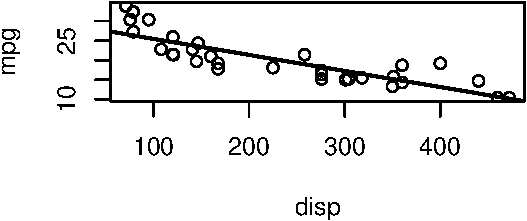
\includegraphics[width=\maxwidth]{figure/slr7-1} 

}

\caption[Linear regression]{Linear regression}\label{fig:slr7}
\end{figure}


\end{knitrout}
\end{frame}



\begin{frame}[fragile]
\frametitle{Include a Table}
\scriptsize
\begin{knitrout}\footnotesize
\definecolor{shadecolor}{rgb}{0.969, 0.969, 0.969}\color{fgcolor}\begin{kframe}
\begin{verbatim}
<<table.ex, results='asis'>>=
library(xtable)
iris[1:5,1:5] %>% 
xtable(caption='Sample of Iris data') %>%
print(include.rownames=FALSE)
@
\end{verbatim}
\end{kframe}
\end{knitrout}
% latex table generated in R 3.6.0 by xtable 1.8-4 package
% Mon May 13 19:33:00 2019
\begin{table}[ht]
\centering
\begin{tabular}{rrrrl}
  \hline
Sepal.Length & Sepal.Width & Petal.Length & Petal.Width & Species \\ 
  \hline
5.10 & 3.50 & 1.40 & 0.20 & setosa \\ 
  4.90 & 3.00 & 1.40 & 0.20 & setosa \\ 
  4.70 & 3.20 & 1.30 & 0.20 & setosa \\ 
  4.60 & 3.10 & 1.50 & 0.20 & setosa \\ 
  5.00 & 3.60 & 1.40 & 0.20 & setosa \\ 
   \hline
\end{tabular}
\caption{Sample of Iris data} 
\end{table}

\end{frame}


\begin{comment}
\section{Details}

\subsection{Code Chunks}

\begin{frame}{A selection of \texttt{knitr} code chunk options}
content...
\end{frame}


\begin{frame}{Set global chunk options}
content...
\end{frame}


\begin{frame}{Option Aliases}
see page 109 yihui
\end{frame}


\begin{frame}{Option Templates}
see page 110 yihui
\end{frame}

\begin{frame}{Chunk References}
see page 79 yihui
\end{frame}


\begin{frame}{Code in Appendix}
see page 110 yihui
\end{frame}



\subsection{Hooks}
\begin{frame}{A selection of \texttt{knitr} code chunk options}
content...
\end{frame}


\subsection{Child Documents}
\begin{frame}{A selection of \texttt{knitr} code chunk options}
see 83
\end{frame}



\subsection{Custom Environments}
\begin{frame}{Example Environment}
see 120
\end{frame}
\end{comment}


\subsection{RMarkdown}

\begin{frame}{Markdown: HTML without knowing HTML}
\begin{center}
	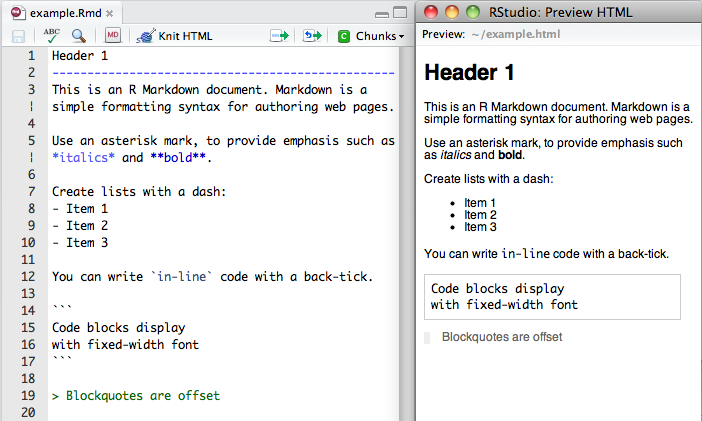
\includegraphics[scale=0.45, keepaspectratio]{markdown}
\end{center}
\end{frame}

\begin{frame}{R + Markdown = RMarkdown}
\begin{center}
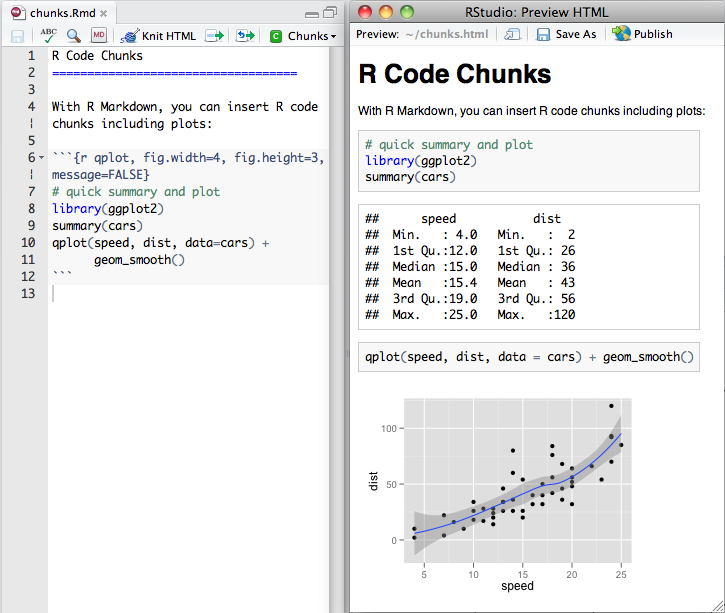
\includegraphics[scale=0.36, keepaspectratio]{rmarkdown}
\end{center}
\end{frame}

\begin{frame}{What \texttt{rmarkdown} does}
\textbf{\code{RMarkdown}} example:

\begin{center}
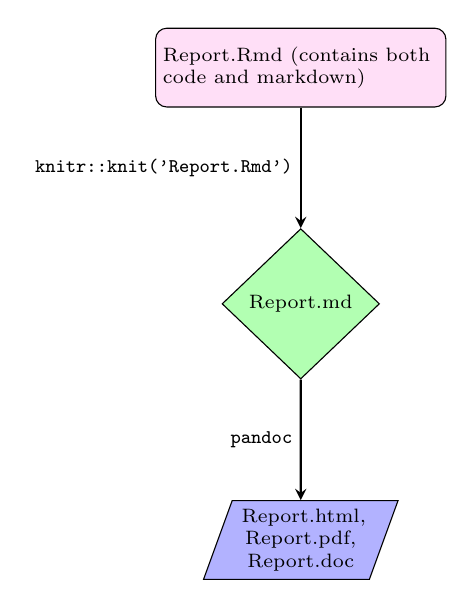
\begin{tikzpicture}
\scriptsize
\node (expr) [startstop] {Report.Rmd (contains both code and markdown)};
\node (science) [decision, below of=expr, xshift=0cm, yshift=-2cm] {Report.md};
\draw [arrow] (expr) -- node[anchor=east]{\texttt{knitr::knit('Report.Rmd')}} (science);
\pause \node (pdf) [io, below of=science, xshift=0cm, yshift=-2cm] {Report.html, Report.pdf, Report.doc};
\draw [arrow] (science) -- node[anchor=east]{\texttt{pandoc}} (pdf);
\end{tikzpicture}
\end{center}
\end{frame}


\begin{frame}\frametitle{Compiling a \texttt{.Rmd} document}

\begin{block}{The two steps on previous slide can be executed in one command:}
\[ \textrm{\texttt{rmarkdown::render()}} \]
\end{block}

or in \texttt{RStudio}:
\begin{figure}[h!]
\centering
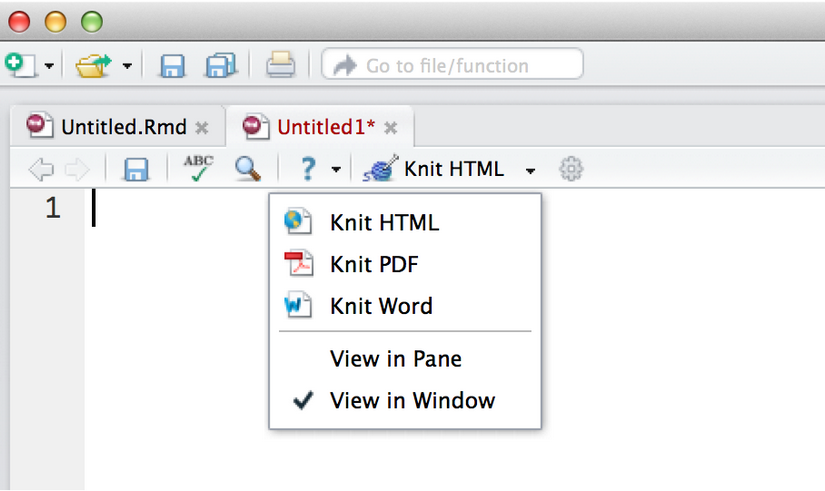
\includegraphics[scale=0.21, keepaspectratio]{rmddrop.png}
\end{figure}
%\textit{Demonstrate:} Explore \texttt{RStudio}, projects and \texttt{.Rprofile}
\end{frame}


\begin{frame}{Comment choisir entre \LaTeX\mbox{ }et Markdown ?}
%\hspace*{-1.9cm}\parbox[t]{\textwidth}{
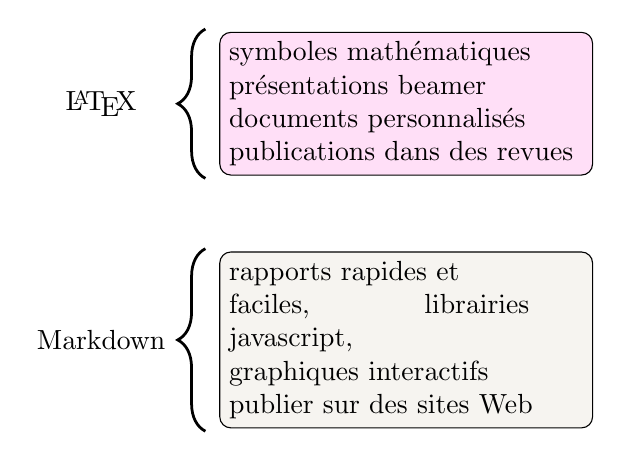
\begin{tikzpicture}
\node (expr) [startstop4] {symboles mathématiques \textcolor{pinkish}{t} présentations beamer  \textcolor{pinkish}{tecc}
	documents personnalisés\textcolor{pinkish}{l} publications dans des revues 
	%\code{getwd()}\textcolor{pinkish}{teccc}
	%\code{rm()}\textcolor{pinkish}{tevvvvvvv}
};
\node (fat) [startstop2, below of=expr, xshift=-.0cm, yshift=-2.0cm] {rapports rapides et faciles,\textcolor{background}{tkkjjjjjjk} 
librairies javascript, \textcolor{background}{tekkhhhht}	graphiques interactifs \textcolor{background}{te} publier sur des sites Web};
%\node (script) [startstop3, below of=fat, xshift=.1cm, yshift=-1.5cm] {
%\code{read.table()}
%\code{write.table()}
%\code{load()}
%\code{save()}\textcolor{beige}{text}
%\code{source()}};
\draw[decoration={brace,raise=5pt, amplitude=10pt},decorate,line width=1pt] 
([yshift=-1pt]expr.south west) -- ([yshift=1pt]expr.north west) node [black,midway,xshift=-1.5cm] 
{ \LaTeX};
\draw[decoration={brace,raise=5pt,amplitude=10pt},decorate,line width=1pt] 
([yshift=-1pt]fat.south west) -- ([yshift=1pt]fat.north west) node [black,midway,xshift=-1.5cm] 
{Markdown};
%\draw[decoration={brace,raise=5pt,amplitude=10pt},decorate,line width=1pt] 
%  ([yshift=-1pt]script.south west) -- ([yshift=1pt]script.north west) node [black,midway,xshift=-3cm] 
{\footnotesize Accéder les données et scripts R};
\end{tikzpicture}
%}
\end{frame}

\subsection{Git et GitHub}

\begin{frame}{Git et GitHub}
\begin{figure}[h!]
	\centering
	\includegraphics[scale=0.28, keepaspectratio]{git-and-github-workflow.png}
\end{figure}
\end{frame}


\section{Exemples}

\subsection{002-minimum-working-example}

\begin{frame}{Minimum Working Example}
\href{https://github.com/sahirbhatnagar/raqc/tree/master/002-minimum-working-example}{https://github.com/sahirbhatnagar/raqc/tree/master/002-minimum-working-example}
\end{frame}


\subsection{003-model-output}

\begin{frame}{Extracting output from Regression Models}
\href{https://github.com/sahirbhatnagar/raqc/tree/master/003-model-output}{https://github.com/sahirbhatnagar/raqc/tree/master/003-model-output}
\end{frame}


\subsection{004-figures}

\begin{frame}{Figures}
\href{https://github.com/sahirbhatnagar/raqc/tree/master/004-figures}{https://github.com/sahirbhatnagar/raqc/tree/master/004-figures}
\end{frame}


\subsection{005-beamer-presentation}

\begin{frame}{Beamer Presentations}
\href{https://github.com/sahirbhatnagar/raqc/tree/master/005-beamer-presentation}{https://github.com/sahirbhatnagar/raqc/tree/master/005-beamer-presentation}
\end{frame}


\subsection{006-sensitivity-analysis-one-parameter}

\begin{frame}{Changing one Parameter in an Analysis}
\href{https://github.com/sahirbhatnagar/raqc/tree/master/006-sensitivity-analysis-one-parameter}{https://github.com/sahirbhatnagar/raqc/tree/master/006-sensitivity-analysis-one-parameter}
\end{frame}

\subsection{007-sensitivity-analysis-many-parameters}

\begin{frame}{Changing Many Parameters in an Analysis}
\href{https://github.com/sahirbhatnagar/raqc/tree/master/007-sensitivity-analysis-many-parameters}{https://github.com/sahirbhatnagar/raqc/tree/master/007-sensitivity-analysis-many-parameters}
\end{frame}


\subsection{008-large-documents}

\begin{frame}{Large Documents}
\href{https://github.com/sahirbhatnagar/raqc/tree/master/008-large-documents}{https://github.com/sahirbhatnagar/raqc/tree/master/008-large-documents}
\end{frame}

\subsection{009-rmarkdown}

\begin{frame}{HTML Reports}
\href{https://github.com/sahirbhatnagar/raqc/tree/master/009-rmarkdown}{https://github.com/sahirbhatnagar/raqc/tree/master/009-rmarkdown}
\end{frame}

\subsection{010-rmarkdown-presentation}

\begin{frame}{HTML Presentations}
\href{https://github.com/sahirbhatnagar/raqc/tree/master/010-rmarkdown-presentation}{https://github.com/sahirbhatnagar/raqc/tree/master/010-rmarkdown-presentation}
\end{frame}



\section{Final Remarks}

\begin{frame}
\begin{figure}[h!]
\centering
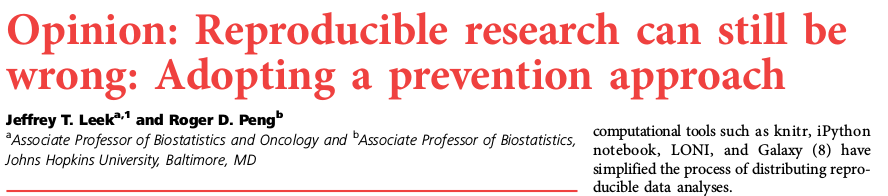
\includegraphics[scale=0.30, keepaspectratio]{./leek}
\end{figure}
\end{frame}

\begin{frame}
\frametitle{Always Remember ...}

\[ \textrm{Reproducibility} \propto \frac{1}{\textrm{copy paste}}  \]


\end{frame}


\begin{frame}{Is the juice worth the squeeze?}
\begin{figure}[h!]
\centering
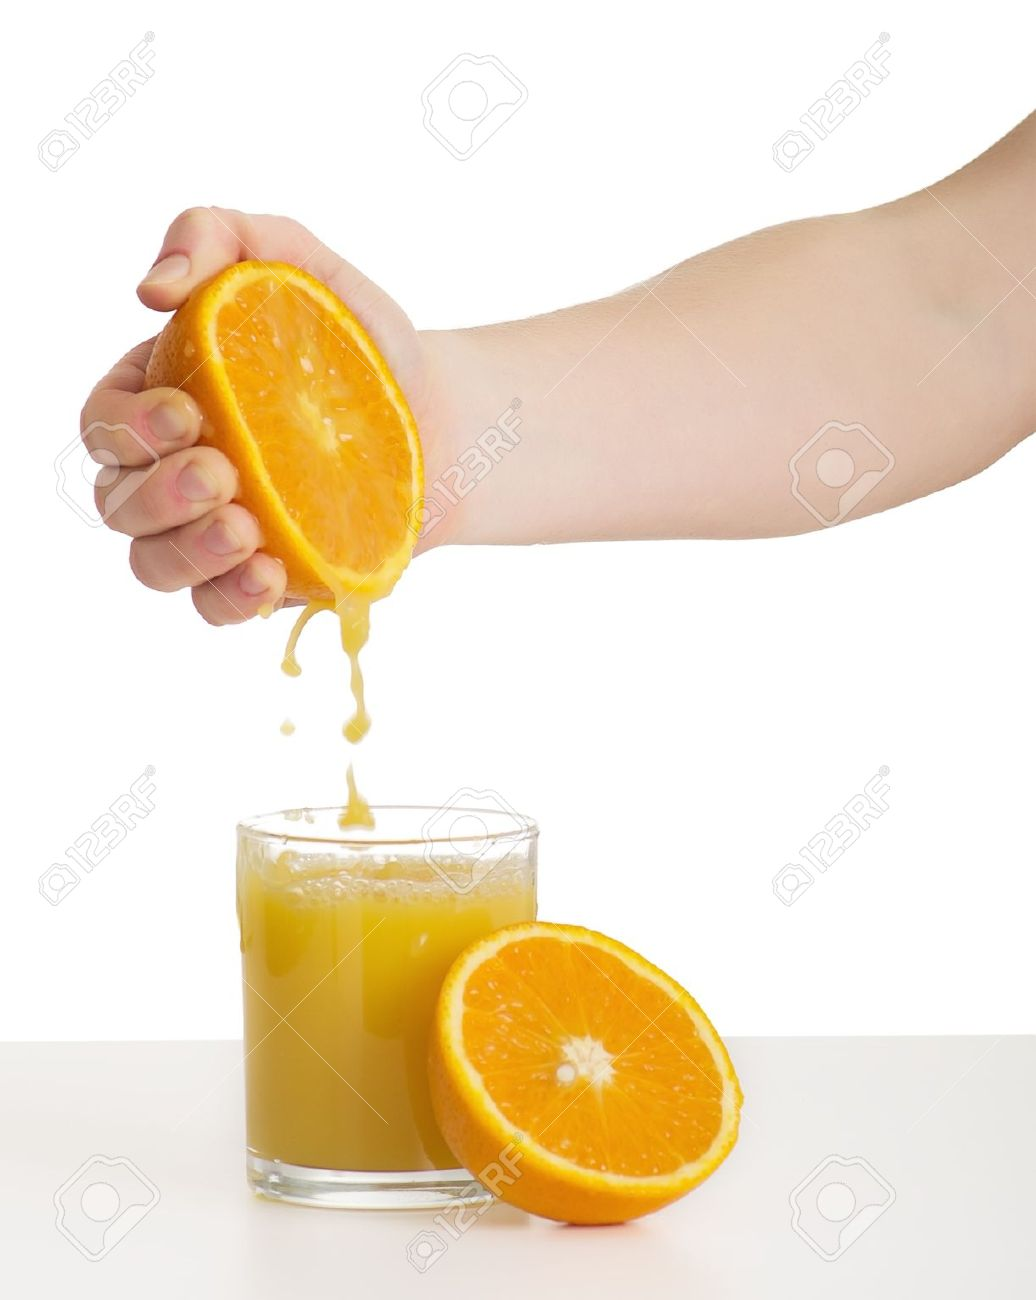
\includegraphics[scale=0.40, keepaspectratio]{./juice}
\end{figure}
\end{frame}

\end{document}

